\section{最优解的判别}
\label{sec:opt-optimality}

前面的条件都是整体性的：可行集是否紧、目标是否凸。实际计算时，我们手里只有一个候选点，以及它附近的函数值和导数。接下来要弄清：只看这一点的导数信息，能断定什么？不能断定什么？主线讨论无约束的光滑目标，或者可行集内部的点；最后说明受约束时情况怎样改变。

全卷用$\nabla f(\bm{x})$表示梯度，$\nabla^2f(\bm{x})$表示Hessian矩阵。多元函数的梯度、Hessian和Taylor公式，可参考\BookChapterRef{chap:multivariate-differentiation}{卷二第20章“多元函数微分”}。

\paragraph{沿每个方向看}
站在最低点上，朝任何方向迈一小步都不会更低。把这句话变成计算：固定点$\bar{\bm{x}}$和方向$\bm{d}$，只看沿这条直线的一元函数
\[
 \phi(t)=f(\bar{\bm{x}}+t\bm{d}).
\]
链式法则给出它在$t=0$处的导数，即沿$\bm{d}$的\term{方向导数}（directional derivative）：
\begin{equation}
 \phi'(0)=\langle\nabla f(\bar{\bm{x}}),\bm{d}\rangle.
 \label{eq:opt-directional-derivative}
\end{equation}

$\phi'(0)<0$时，沿$\bm{d}$走一小步目标下降，这样的$\bm{d}$称为\term{下降方向}（descent direction）。条件$\langle\nabla f(\bar{\bm{x}}),\bm{d}\rangle<0$说明，只要梯度不为零，下降方向就占据整整半个空间，分界面与梯度垂直，也就是等高线在该点的切线。

用实例~\eqref{eq:opt-ridge-instance}取$\gamma=0.5$算一次。梯度的两个分量是
\[
 \frac{\partial f}{\partial x_1}=x_1+x_2-2+\gamma x_1,\qquad
 \frac{\partial f}{\partial x_2}=x_1+x_2-2+\gamma x_2.
\]
在$\bar{\bm{x}}=(2,0)$处，$\nabla f(\bar{\bm{x}})=(1,0)$。取$\bm{d}=(-1,1)$，由式~\eqref{eq:opt-directional-derivative}，方向导数是$-1$。

直接验证一下。沿这个方向$x_1+x_2$保持为$2$，拟合项为零，于是
\[
 \phi(t)=\frac14\bigl((2-t)^2+t^2\bigr),\qquad\phi'(0)=\frac14\cdot(-4)=-1.
\]
两种算法结果相同。图~\ref{fig:opt-descent-halfplane}中，浅绿半平面是全部下降方向，竖直虚线是等高线在$\bar{\bm{x}}$处的切线。负梯度方向$-\nabla f$是其中的一个，$\bm{d}$是另一个，后者比负梯度更接近指向红色最优解的方向。

\begin{BookInlineFigure}
  \centering
  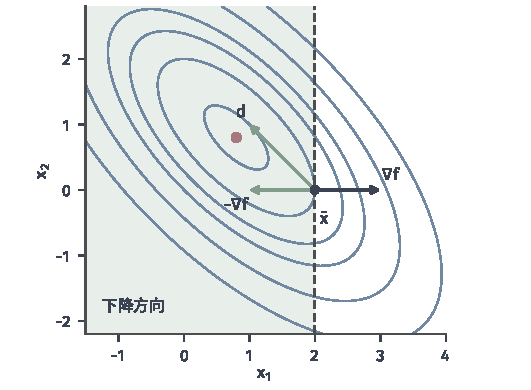
\includegraphics[width=90mm]{figures/05-optimization/01-linear-programming/matplotlib/opt-descent-halfplane/figure.pdf}
  \caption{下降方向构成半平面。蓝线是$f(\bm{x})=\frac12(x_1+x_2-2)^2+\frac14\lVert\bm{x}\rVert_2^2$的等高线，$\bar{\bm{x}}=(2,0)$处的梯度为$(1,0)$。竖直虚线与梯度垂直，浅绿区域的方向都满足$\langle\nabla f(\bar{\bm{x}}),\bm{d}\rangle<0$。绿色箭头是负梯度方向和$\bm{d}=(-1,1)$，红点是最优解$(0.8,0.8)$。}
  \label{fig:opt-descent-halfplane}
\end{BookInlineFigure}

\paragraph{一阶必要条件}
若$\bar{\bm{x}}$是局部最优解，并且各个方向都可以走，就不能有下降方向。半个空间都是下降方向的唯一例外是梯度为零。为了让“各个方向都可以走”成立，下面要求点在可行集内部：称$\bar{\bm{x}}$是$\bm{C}$的\term{内点}（interior point），如果存在$r>0$使$\bm{B}(\bar{\bm{x}},r)\subseteq\bm{C}$。

\begin{theorem}[一阶必要条件]
\label{thm:opt-first-order}
设$\bm{x}^\star$是$\bm{C}$的内点，$f$在$\bm{x}^\star$处可微。若$\bm{x}^\star$是$f$在$\bm{C}$上的局部最优解，则
\begin{equation}
 \nabla f(\bm{x}^\star)=\bm{0}.
 \label{eq:opt-first-order}
\end{equation}
\end{theorem}

\begin{proof}
任取方向$\bm{d}$。$\lvert t\rvert$充分小时，$\bm{x}^\star+t\bm{d}$既在$\bm{C}$内，又在局部最优的邻域内，所以$\phi(t)=f(\bm{x}^\star+t\bm{d})\geq\phi(0)$。

当$t>0$时，$(\phi(t)-\phi(0))/t\geq0$。令$t\downarrow0$，由式~\eqref{eq:opt-directional-derivative}得到
\[
 \langle\nabla f(\bm{x}^\star),\bm{d}\rangle\geq0.
\]
这对任意方向成立。取$\bm{d}=-\nabla f(\bm{x}^\star)$，得到$-\lVert\nabla f(\bm{x}^\star)\rVert_2^2\geq0$，所以梯度为零。
\end{proof}

梯度为零的点称为\term{驻点}（stationary point）。这个条件只是必要的，它在三处不能往下推。第一，驻点不一定是最小点：$x_1^2-x_2^2$在原点有驻点，沿$x_1$轴是最低点，沿$x_2$轴是最高点，这样的驻点称为\term{鞍点}（saddle point）。第二，定理只管内点：例子~\ref{ex:opt-local-global}的全局最优解$x=1.5$在边界上，导数不为零。第三，即使驻点是局部最优，也可能不是全局最优。

下面的二维例子同时展示这几点，后面会反复用到。考虑$\mathbb{R}^2$上的
\begin{equation}
 f(\bm{x})=x_1^3-3x_1+x_2^2.
 \label{eq:opt-cubic}
\end{equation}
令梯度为零：
\[
 \nabla f(\bm{x})=(3x_1^2-3,\ 2x_2)=\bm{0}.
\]
解得两个驻点$(1,0)$和$(-1,0)$。一阶信息到此为止，分不出这两个点的差别。

\paragraph{凸目标的驻点}
凸性能把必要条件变成充分条件。关键在于：凸函数的图像不仅在弦下方，还在每一点切线的上方。切线只用到一个点的函数值和梯度，它若是全局下界，单点信息就能告诉我们远处的目标至少有多大。

\begin{theorem}[一阶支撑不等式]
\label{thm:opt-support}
设$\bm{D}\subseteq\mathbb{R}^n$是开凸集，$f:\bm{D}\to\mathbb{R}$可微。$f$是凸函数，当且仅当对任意$\bm{u},\bm{v}\in\bm{D}$，
\begin{equation}
 f(\bm{v})\geq f(\bm{u})+\langle\nabla f(\bm{u}),\bm{v}-\bm{u}\rangle.
 \label{eq:opt-support}
\end{equation}
\end{theorem}

\begin{proof}
设$f$凸。对$t\in(0,1]$，由式~\eqref{eq:opt-convex-function}，
\[
 f\bigl(\bm{u}+t(\bm{v}-\bm{u})\bigr)\leq(1-t)f(\bm{u})+tf(\bm{v}).
\]
移项并除以$t$，得到
\[
 \frac{f\bigl(\bm{u}+t(\bm{v}-\bm{u})\bigr)-f(\bm{u})}{t}\leq f(\bm{v})-f(\bm{u}).
\]
令$t\downarrow0$，左端趋于方向导数$\langle\nabla f(\bm{u}),\bm{v}-\bm{u}\rangle$，即得式~\eqref{eq:opt-support}。

反过来，设式~\eqref{eq:opt-support}成立。取$\bm{z}=\theta\bm{u}+(1-\theta)\bm{v}$，以$\bm{z}$为切点，分别写出
\[
 f(\bm{u})\geq f(\bm{z})+\langle\nabla f(\bm{z}),\bm{u}-\bm{z}\rangle,\qquad
 f(\bm{v})\geq f(\bm{z})+\langle\nabla f(\bm{z}),\bm{v}-\bm{z}\rangle.
\]
第一式乘$\theta$，第二式乘$1-\theta$，再相加。由$\bm{z}$的定义，
\[
 \theta(\bm{u}-\bm{z})+(1-\theta)(\bm{v}-\bm{z})=\bm{0},
\]
所以内积项抵消，得到式~\eqref{eq:opt-convex-function}。
\end{proof}

图~\ref{fig:opt-support-tangent}对比了两种情形。凸函数的切线（紫色）整条位于图像下方，是全局的下界。非凸函数在$x=0$处的水平切线则位于图像上方的一大段区域，单点信息不能给出下界。

\begin{BookInlineFigure}
  \centering
  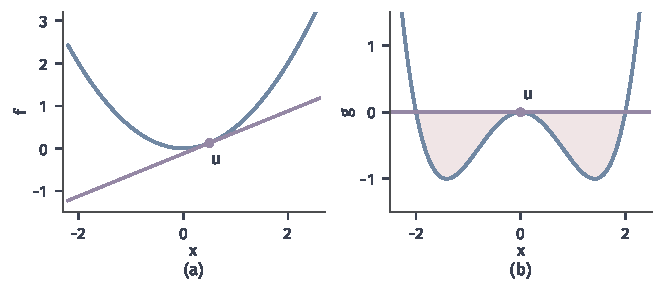
\includegraphics[width=112mm]{figures/05-optimization/01-linear-programming/matplotlib/opt-support-tangent/figure.pdf}
  \caption{切线是否是全局下界。(a)凸函数$f(x)=x^2/2$在$u=1/2$处的紫色切线整条位于图像下方。(b)非凸函数$g(x)=x^4/4-x^2$在$u=0$处的切线是水平线，在$0<\lvert x\rvert<2$时位于图像上方（浅红区域），不是下界。}
  \label{fig:opt-support-tangent}
\end{BookInlineFigure}

把$\nabla f(\bm{x}^\star)=\bm{0}$代入式~\eqref{eq:opt-support}，水平的切平面把最小值钉在切点上。

\begin{theorem}[凸目标驻点的全局最优性]
\label{thm:opt-convex-stationary}
设$\bm{D}$是开凸集，$f:\bm{D}\to\mathbb{R}$凸且可微。则$\bm{x}^\star\in\bm{D}$是$f$在$\bm{D}$上的全局最优解，当且仅当$\nabla f(\bm{x}^\star)=\bm{0}$。
\end{theorem}

\begin{proof}
必要性来自定理~\ref{thm:opt-first-order}，开集中每个点都是内点。充分性：若梯度为零，由式~\eqref{eq:opt-support}，对任意$\bm{v}\in\bm{D}$，
\[
 f(\bm{v})\geq f(\bm{x}^\star)+\langle\bm{0},\bm{v}-\bm{x}^\star\rangle=f(\bm{x}^\star).
\]
\end{proof}

这个结论的价值在于：对凸目标，求解优化问题等价于解方程$\nabla f=\bm{0}$，找到的任何一个解都是全局最优。二次拟合~\eqref{eq:opt-ridge}的梯度是
\begin{equation}
 \nabla f(\bm{x})=\bm{A}^\top(\bm{A}\bm{x}-\bm{b})+\gamma\bm{x},
 \label{eq:opt-ridge-gradient}
\end{equation}
驻点条件就是正规方程
\[
 (\bm{A}^\top\bm{A}+\gamma\bm{I})\bm{x}=\bm{A}^\top\bm{b}.
\]
实例中它化为
\[
 (1+\gamma)x_1+x_2=2,\qquad x_1+(1+\gamma)x_2=2.
\]
两式相减得$\gamma(x_1-x_2)=0$。$\gamma>0$时$x_1=x_2$，解出的正是式~\eqref{eq:opt-ridge-solution}；$\gamma=0$时两式都是$x_1+x_2=2$，解成一条直线。

强凸函数还多一个二次项。设$f$可微且$\mu$强凸。由式~\eqref{eq:opt-strong-equivalent}，$f-\frac{\mu}{2}\lVert\cdot\rVert_2^2$是凸函数，它的梯度是$\nabla f(\bm{x})-\mu\bm{x}$。对它用式~\eqref{eq:opt-support}，其中多出的项可以合并：
\[
 \lVert\bm{v}\rVert_2^2-\lVert\bm{u}\rVert_2^2-2\langle\bm{u},\bm{v}-\bm{u}\rangle=\lVert\bm{v}-\bm{u}\rVert_2^2.
\]
于是得到
\begin{equation}
 f(\bm{v})\geq f(\bm{u})+\langle\nabla f(\bm{u}),\bm{v}-\bm{u}\rangle+\frac{\mu}{2}\lVert\bm{v}-\bm{u}\rVert_2^2.
 \label{eq:opt-strong-support}
\end{equation}

这个不等式顺便补上了强凸目标的存在性。在$\mathbb{R}^n$上取$\bm{u}=\bm{0}$，由柯西不等式，
\[
 f(\bm{v})\geq f(\bm{0})-\lVert\nabla f(\bm{0})\rVert_2\lVert\bm{v}\rVert_2+\frac{\mu}{2}\lVert\bm{v}\rVert_2^2.
\]
右端在$\lVert\bm{v}\rVert_2\to\infty$时趋于$+\infty$，所以$f$强制。可微函数连续，由上一节的结论，最优解存在。再由定理~\ref{thm:opt-quadratic-growth}，最优解唯一。

\paragraph{二阶条件：曲率区分驻点的类型}
一阶条件分不清极小、极大与鞍点，因为驻点处梯度项消失了，函数的变化由下一阶主导。设$f$二阶连续可微，$\nabla f(\bm{x}^\star)=\bm{0}$。由带Lagrange余项的Taylor公式，对小的$\bm{h}$，存在$s\in(0,1)$使
\begin{equation}
 f(\bm{x}^\star+\bm{h})-f(\bm{x}^\star)=\frac12\bm{h}^\top\nabla^2f(\bm{x}^\star+s\bm{h})\bm{h}.
 \label{eq:opt-taylor}
\end{equation}
量$\bm{d}^\top\nabla^2f(\bm{x}^\star)\bm{d}$是函数沿$\bm{d}$方向的曲率：为正时向上弯，为负时向下弯。

\begin{theorem}[二阶条件]
\label{thm:opt-second-order}
设$\bm{x}^\star$是$\bm{C}$的内点，$f$在$\bm{x}^\star$附近二阶连续可微。
\begin{enumerate}
 \item 必要条件：若$\bm{x}^\star$是局部最优解，则$\nabla f(\bm{x}^\star)=\bm{0}$且$\nabla^2f(\bm{x}^\star)$半正定。
 \item 充分条件：若$\nabla f(\bm{x}^\star)=\bm{0}$且$\nabla^2f(\bm{x}^\star)$正定，则$\bm{x}^\star$是严格局部最优解。
\end{enumerate}
\end{theorem}

\begin{proof}
记$\bm{H}=\nabla^2f(\bm{x}^\star)$。先证必要条件，一阶部分即定理~\ref{thm:opt-first-order}。假设某个$\bm{d}$使$\bm{d}^\top\bm{H}\bm{d}<0$。由Hessian的连续性，$\lvert t\rvert$充分小时，对所有$s\in(0,1)$都有
\[
 \bm{d}^\top\nabla^2f(\bm{x}^\star+st\bm{d})\bm{d}<0.
\]
在式~\eqref{eq:opt-taylor}中取$\bm{h}=t\bm{d}$，就得到$f(\bm{x}^\star+t\bm{d})<f(\bm{x}^\star)$，与局部最优矛盾。

再证充分条件。记$\lambda_{\min}>0$为$\bm{H}$的最小特征值，于是
\[
 \bm{h}^\top\bm{H}\bm{h}\geq\lambda_{\min}\lVert\bm{h}\rVert_2^2.
\]
由Hessian的连续性，取足够小的$r>0$，使$\bm{B}(\bm{x}^\star,r)\subseteq\bm{C}$，并且$\lVert\bm{h}\rVert_2<r$时
\[
 \bigl\lVert\nabla^2f(\bm{x}^\star+\bm{h})-\bm{H}\bigr\rVert_2\leq\frac{\lambda_{\min}}{2}.
\]

这样对$\lVert\bm{h}\rVert_2<r$和任意$s\in(0,1)$，二次型至多比$\bm{h}^\top\bm{H}\bm{h}$小$\frac{\lambda_{\min}}{2}\lVert\bm{h}\rVert_2^2$。代入式~\eqref{eq:opt-taylor}，对$\bm{h}\neq\bm{0}$，
\[
 f(\bm{x}^\star+\bm{h})-f(\bm{x}^\star)\geq\frac12\Bigl(\lambda_{\min}-\frac{\lambda_{\min}}{2}\Bigr)\lVert\bm{h}\rVert_2^2=\frac{\lambda_{\min}}{4}\lVert\bm{h}\rVert_2^2>0.
\]
所以$\bm{x}^\star$是严格局部最优解。
\end{proof}

回到式~\eqref{eq:opt-cubic}。它的Hessian是
\[
 \nabla^2f(\bm{x})=\begin{bmatrix}6x_1&0\\0&2\end{bmatrix}.
\]
在$(1,0)$处是$\operatorname{diag}(6,2)$，正定，所以这是严格局部最优解，函数值为$-2$。在$(-1,0)$处是$\operatorname{diag}(-6,2)$，不定，不是局部最优解，也不是局部极大点，而是鞍点，函数值为$2$。

二阶条件到此仍是局部结论。沿$x_1\to-\infty$，$f\to-\infty$，所以这个问题无下界，局部最优点$(1,0)$远不是全局最优。图~\ref{fig:opt-cubic-stationary}中，穿过鞍点的粗等高线围出一个“盆”，$(1,0)$在盆底，翻过鞍点向左，地面一路下降。

\begin{BookInlineFigure}
  \centering
  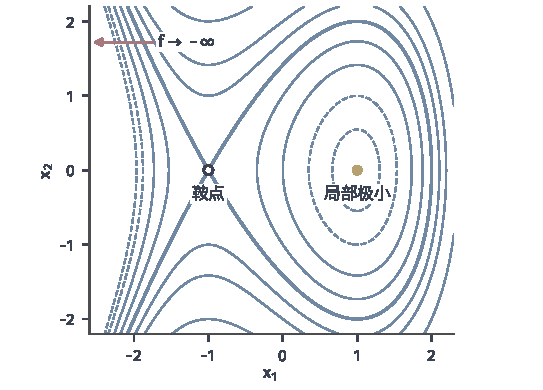
\includegraphics[width=92mm]{figures/05-optimization/01-linear-programming/matplotlib/opt-cubic-stationary/figure.pdf}
  \caption{$f(\bm{x})=x_1^3-3x_1+x_2^2$的等高线，虚线是负值水平。黄点$(1,0)$是严格局部最优解，空心点$(-1,0)$是鞍点，粗线是穿过鞍点的等高线$f=2$。红色箭头所指的左侧目标趋于$-\infty$，所以局部最优解不是全局最优解。}
  \label{fig:opt-cubic-stationary}
\end{BookInlineFigure}

要从局部曲率得到整体结论，就得要求曲率处处非负，这正是凸性的二阶判据。

\begin{theorem}[凸性的二阶判据]
\label{thm:opt-hessian-convex}
设$\bm{D}\subseteq\mathbb{R}^n$是开凸集，$f:\bm{D}\to\mathbb{R}$二阶连续可微。则$f$凸当且仅当$\nabla^2f(\bm{x})$在$\bm{D}$上处处半正定；$f$是$\mu$强凸的当且仅当$\nabla^2f(\bm{x})-\mu\bm{I}$在$\bm{D}$上处处半正定。
\end{theorem}

\begin{proof}
设$f$凸，取$\bm{x}\in\bm{D}$和方向$\bm{h}$。$t$充分小时，由式~\eqref{eq:opt-support}和带Lagrange余项的Taylor公式，存在$s\in(0,1)$使
\[
 0\leq f(\bm{x}+t\bm{h})-f(\bm{x})-t\langle\nabla f(\bm{x}),\bm{h}\rangle=\frac{t^2}{2}\bm{h}^\top\nabla^2f(\bm{x}+st\bm{h})\bm{h}.
\]
除以$t^2/2$，令$t\to0$，由Hessian的连续性得到$\bm{h}^\top\nabla^2f(\bm{x})\bm{h}\geq0$。

反过来，设Hessian处处半正定。对$\bm{u},\bm{v}\in\bm{D}$，令$\psi(t)=f(\bm{u}+t(\bm{v}-\bm{u}))$，则$\psi''\geq0$。由带Lagrange余项的Taylor公式，
\[
 \psi(1)=\psi(0)+\psi'(0)+\frac12\psi''(\xi)\geq\psi(0)+\psi'(0),
\]
这正是式~\eqref{eq:opt-support}，由定理~\ref{thm:opt-support}，$f$凸。

强凸的情形，把上述结论用于$f-\frac{\mu}{2}\lVert\cdot\rVert_2^2$，它的Hessian是$\nabla^2f-\mu\bm{I}$，再用式~\eqref{eq:opt-strong-equivalent}。
\end{proof}

判据要求在整个开凸集上成立，只在单个点检查不能证明函数凸。式~\eqref{eq:opt-cubic}在$(1,0)$处Hessian正定，但在$x_1<0$处有负特征值，所以它不是凸函数，局部最优也就不必是全局最优。二次拟合的Hessian处处等于$\bm{A}^\top\bm{A}+\gamma\bm{I}$，半正定，这与前面用弦算出的结论一致。

\paragraph{退化驻点：二阶也判不了}
定理~\ref{thm:opt-second-order}的两个条件之间留有缺口：Hessian半正定但奇异时，必要条件满足，充分条件不满足，二阶信息不足以判断。这样的驻点称为\term{退化驻点}（degenerate stationary point）。

函数$x_1^2+x_2^4$和$x_1^2+x_2^3$在原点的梯度都为零，Hessian都是$\operatorname{diag}(2,0)$，二阶信息完全相同。前者对$\bm{x}\neq\bm{0}$恒为正，原点是严格最小点，说明正定不是必要的。后者沿$(0,-t)$取值$-t^3<0$，原点不是局部最优解，说明半正定不是充分的。

决定结果的是$x_2$方向的高阶项，这正是Hessian在零特征方向上看不到的信息。图~\ref{fig:opt-stationary-types}中，请注意红色区域是否碰到原点：碰到就说明任意小的邻域里都有更低的点。(c)与(d)的二阶信息相同，红色区域却一有一无。

\begin{BookInlineFigure}
  \centering
  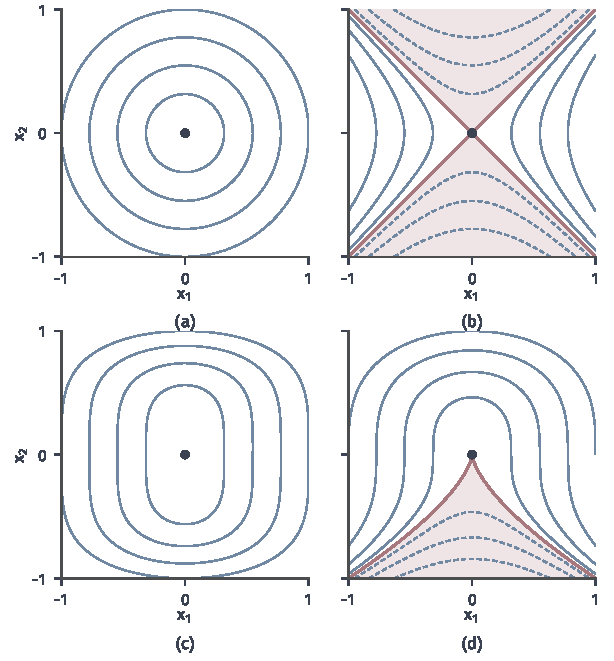
\includegraphics[width=104mm]{figures/05-optimization/01-linear-programming/matplotlib/opt-stationary-types/figure.pdf}
  \caption{原点处四种驻点的等高线，浅红区域是函数值低于$f(\bm{0})=0$的点，虚线是负值水平，红线是零等高线。(a)$x_1^2+x_2^2$，Hessian正定，严格最小点。(b)$x_1^2-x_2^2$，Hessian不定，鞍点。(c)$x_1^2+x_2^4$，Hessian为$\operatorname{diag}(2,0)$，仍是严格最小点。(d)$x_1^2+x_2^3$，Hessian同为$\operatorname{diag}(2,0)$，但原点下方有更低的点，不是局部最优解。}
  \label{fig:opt-stationary-types}
\end{BookInlineFigure}

\paragraph{负曲率方向}
定理~\ref{thm:opt-second-order}必要性的证明还包含一条可以操作的信息。若驻点处存在方向$\bm{d}$使$\bm{d}^\top\nabla^2f(\bm{x}^\star)\bm{d}<0$，就称$\bm{d}$为\term{负曲率方向}（negative curvature direction）。沿它走，一阶变化为零，目标却以二次速度下降。

对$f(\bm{x})=x_1^2-x_2^2$，Hessian是$\operatorname{diag}(2,-2)$。沿单位方向$\bm{d}$，
\[
 f(t\bm{d})=\frac{t^2}{2}\bm{d}^\top\operatorname{diag}(2,-2)\bm{d}=t^2(d_1^2-d_2^2).
\]
图~\ref{fig:opt-saddle-curvature}取三个方向：$\bm{d}_1=(1,0)$曲率为$2$，向上弯；$\bm{d}_2=(1,1)/\sqrt2$曲率为$0$，二阶项恰好消失；$\bm{d}_3=(0,1)$曲率为$-2$，向下弯。站在鞍点上，梯度指不出任何下降方向，Hessian的负特征向量却指出了一条。怎样利用这一点离开鞍点，由第~\ref{chap:saddle-points}章讨论。

\begin{BookInlineFigure}
  \centering
  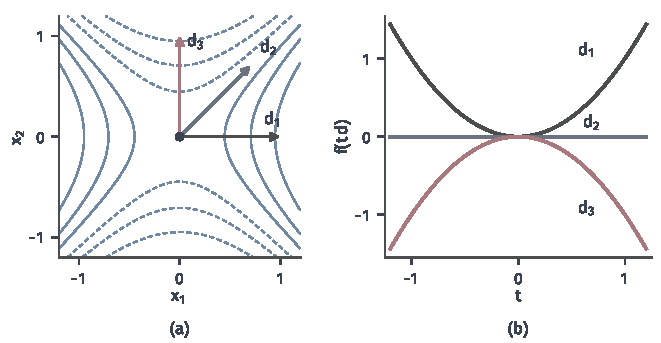
\includegraphics[width=112mm]{figures/05-optimization/01-linear-programming/matplotlib/opt-saddle-curvature/figure.pdf}
  \caption{鞍点处不同方向的曲率。(a)$f(\bm{x})=x_1^2-x_2^2$的等高线（虚线为负值）与三个单位方向。(b)沿这三个方向的一元限制$f(t\bm{d})$：$\bm{d}_1$向上弯，$\bm{d}_2$保持为零，红色的$\bm{d}_3$向下弯，是负曲率方向。}
  \label{fig:opt-saddle-curvature}
\end{BookInlineFigure}

表~\ref{tab:opt-tests}整理到目前为止的判别依据。阅读时要注意“必要”与“充分”的方向，以及结论是局部的还是全局的。

\begin{BookInlineTable}
  \centering
  \begin{tabular}{@{}lll@{}}
    \toprule
    依据 & 性质 & 能得到的结论\\
    \midrule
    $\nabla f=\bm{0}$ & 内点局部最优的必要条件 & 排除非驻点\\
    $\nabla f=\bm{0}$，$\nabla^2f\succeq\bm{0}$ & 局部最优的必要条件 & 进一步排除负曲率点\\
    $\nabla f=\bm{0}$，$\nabla^2f\succ\bm{0}$ & 充分条件，非必要 & 严格局部最优\\
    $\nabla f=\bm{0}$，目标凸 & 充要条件 & 全局最优\\
    \bottomrule
  \end{tabular}
  \caption{无约束光滑目标的判别依据。前三行只看一个点，第四行需要目标的整体性质。}
  \label{tab:opt-tests}
\end{BookInlineTable}

\paragraph{受约束时允许的方向变了}
一阶条件的证明要求$\bm{d}$和$-\bm{d}$都能走。在边界上这个前提不成立，能走的方向变少，要求也相应放宽。称$\bm{d}$是$\bar{\bm{x}}\in\bm{C}$处的\term{可行方向}（feasible direction），如果$t>0$充分小时$\bar{\bm{x}}+t\bm{d}\in\bm{C}$。重复定理~\ref{thm:opt-first-order}证明的前半段，只用$t>0$，就得到：若$\bm{x}^\star$是局部最优解，$f$在该点可微，则对每个可行方向$\bm{d}$，
\begin{equation}
 \langle\nabla f(\bm{x}^\star),\bm{d}\rangle\geq0.
 \label{eq:opt-feasible-direction}
\end{equation}

用资源分配验证。在$\bm{x}^\star=(2,2)$处，两条资源约束取等号，$\bm{d}$可行当且仅当它不增加这两个约束，即
\[
 d_1+d_2\leq0,\qquad 2d_1+d_2\leq0.
\]
目标的梯度是$(-3,-2)$，不等于零。方向导数却可以拆开：
\[
 \langle\nabla f(\bm{x}^\star),\bm{d}\rangle=-3d_1-2d_2=-(d_1+d_2)-(2d_1+d_2)\geq0.
\]

这里的拆分仍然是第~\ref{sec:opt-formulation}节那个“两条约束相加”。图~\ref{fig:opt-boundary-directions}显示了几何含义：$-\nabla f$指向利润增大的方向，它伸出了可行集，而所有绿色的可行方向都和它成钝角或直角。所以$(2,2)$处梯度不为零，却没有“既可行又下降”的方向。

\begin{BookInlineFigure}
  \centering
  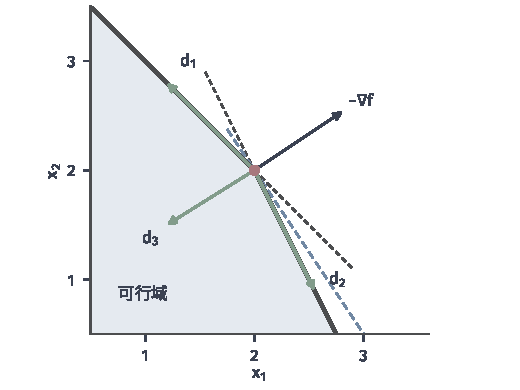
\includegraphics[width=88mm]{figures/05-optimization/01-linear-programming/matplotlib/opt-boundary-directions/figure.pdf}
  \caption{边界上的最优点梯度不必为零。红点是资源分配的最优解$(2,2)$，深灰粗线是两条取等号的约束，蓝色虚线是过该点的等目标线。绿色箭头是可行方向，全部可行方向都夹在$\bm{d}_1=(-1,1)$与$\bm{d}_2=(1,-2)$之间。$-\nabla f=(3,2)$伸出可行集，与每个可行方向的内积都不为正。}
  \label{fig:opt-boundary-directions}
\end{BookInlineFigure}

若$\bm{C}$凸、$f$在包含$\bm{C}$的开凸集上凸且可微，式~\eqref{eq:opt-feasible-direction}对每个$\bm{d}=\bm{y}-\bm{x}^\star$（$\bm{y}\in\bm{C}$）成立时，代入式~\eqref{eq:opt-support}就得到$f(\bm{y})\geq f(\bm{x}^\star)$，所以它也是充分的。

式~\eqref{eq:opt-feasible-direction}还不是一个能直接检验的判据。可行方向可能有无穷多个，曲线边界上甚至可能一个非零的都没有：单位圆周上，沿任何直线都会立刻离开圆周。把它写成关于约束函数的代数条件需要新工具，第~\ref{chap:constrained-optimality}章在明确约束之后建立这些判别。
